%\documentclass{article}
%\usepackage[spanish]{babel}
%\usepackage{amssymb, amsmath} %Paquetes matemáticos de la American Mathematical Society
%\usepackage{graphicx}
%\usepackage[%
%    a4paper,       % Tamaño de papel
%    left=2.5cm,    % Margen izquierdo
%    right=2.5cm,   % Margen derecho
%    top=3cm,       % Margen superior
%    bottom=3cm,    % Margen inferior
%    footskip=1.5cm % Espacio para el pie de página
%]{geometry}
%\usepackage{fancyhdr}
%\pagestyle{fancy}
%\fancyhf{}
%\lhead[\leftmark]{Síntesis de Redes Activas - Laboratorio 1}
%\rfoot[]{\thepage}
%\begin{document}

\section{Circuito III: RECTIFICADOR DE PRECISIÓN }

\subsection{Esquemático y datos}
Se realiza el análisis teórico del circuito que se muestra en la siguiente figura: 
\begin{figure}[h!]
     \centering
     \includegraphics[width=0.5\linewidth]{esquematico3.png}
	 \caption{Esquematico del circuito N° 3}
	 \label{fig:esquematico3}
 \end{figure}
 
Este circuito tiene la funcionalidad de rectificación de una onda de entrada, en un ciclo conduce uno de los diodos, y en el otro ciclo, el otro diodo.

\vspace{1em}

\textbf {Datos: }

\begin{itemize}
  \item Amplificador operacional: LM324
  \item $V_{cc} =10V \quad V_{ss} =-10V$
  \item $D_1 = D_2 =1N4148$
  \item $R_1 = R_3 = R_4 = 10K\Omega \quad 1\% \quad y R_2 = 5K\Omega \quad 1\% $
\end{itemize}

\vspace{1em}

\subsection{Análisis teórico}
Suponiendo que ambos AO son ideales, al igual que los diodos, se analizarán las siguientes relaciones:

\subsubsection{ $V_{o1} = f(V_{in} \quad con \quad 0V < V_{in}) $}

Para este análisis se pasiva el AO U1B. En este caso el diodo que se polariza directamente es el D2, mientras que D1 está polarizado inversamente, actuando como un circuito abierto.

\[V_{in} = V^+ =V^- \]

Como se cierra el lazo por D2, entonces $V_o = V_{in} + 0.7V $

\vspace{1em}

\subsubsection{ $V_{o2} = f(V_{in} \quad con \quad 0V < V_{in}) $}

En este caso se pasiva U1A

\[V_{in} = V_{o2} \frac {R_1 +R_2}{R_1 + R_2 + R_4} = V_{o2} \frac{15k\Omega}{25k\Omega}\]

\[V_{o2}=V_{in}\frac{5}{3} \]

Ahora, pasivando U1B:
\[ \frac{V_{o2}}{R_4} =- \frac{V_{in}}{R_1 + R_2} \]

%\[V_{o2}= -10k\Omega \frac{V_{in}}{15k\Omega} \]

Por superposición: 

\[ V_{o2} =V_{in}(\frac{5-2}{3}) = V_{in}\]

\vspace{1em}

\subsubsection{ $V_{o1} = f(V_{in} \quad con \quad 0V > V_{in}) $}

En esta instancia, el diodo D1 es el que polariza directamente para poder determinar la salida $V_{o1}$ y D2 actua como un circuito abierto.
Se pasiva el AO U1B y tomando $V_x = V_{o1} - 0,7V $:

\[ \frac{0V -V_{in}}{R_3} = \frac{V_{in}-V_x}{R_1} \quad  \Rightarrow \frac{V_{in}}{10k\Omega} = \frac{V_{in}-V_x}{10k\Omega}\]

\[ 2V_{in} = V_x \quad  \Rightarrow \quad 2V_{in}=V_{o1} -0,7V \]

\[ V_{o1} = V_{in} + 0,7V \]

\vspace{1em}

\subsubsection{ $V_{o2} = f(V_{in} \quad con \quad 0V > V_{in}) $}

Se pasiva U1A nuevamente y se calcula  $V_{o2} = f(V_{in} $:

\[V_{in}= V_{o2}\frac{R_2}{R_2 + R_4} \quad  \Rightarrow V_{in} = V_{o2} \frac{5k\Omega}{15k\Omega} \]

\[V_{o2}= 3V_{in} \]

La influencia de U1A en $V_{o2}$ y tomando nuevamente $V_x = V_{o1} - 0,7V $:

\[ \frac{V_x}{R_2} = -\frac{V_{o2}}{R_4} \quad  \Rightarrow \frac{V_{o1}- 0.7V}{5k\Omega} = -\frac{V_{o2}}{10k\Omega} \]

\[ \frac{2V_{in}}{5k\Omega} = -\frac{V_{o2}}{10k\Omega} \]

\[ V_{o2} = -4V_{in} \]

Por superposición:

\[ V_{o2} =V_{in} (3-4) \quad  \Rightarrow V_{o2}= -V_{in} \]

\vspace{1em}

El análisis realizado sugiere el trabajo de un rectificador de onda completa, cuando la señal de entrada es positiva, la salida también lo es,
 y cuando la señal de entrada es negativa, la salida es postiva. La amplitud de salida es igual a la de entrada para ambos casos.

\subsection{Simulación y mediciones de laboratorio}

Utilizando el simulador LTSpice y armando el circuito en físico, se mostrarán las gráficas simuladas y medidas para distintos valores de $V_{in}$:

\vspace{1em}

  \begin{figure}[h!]
     \centering
     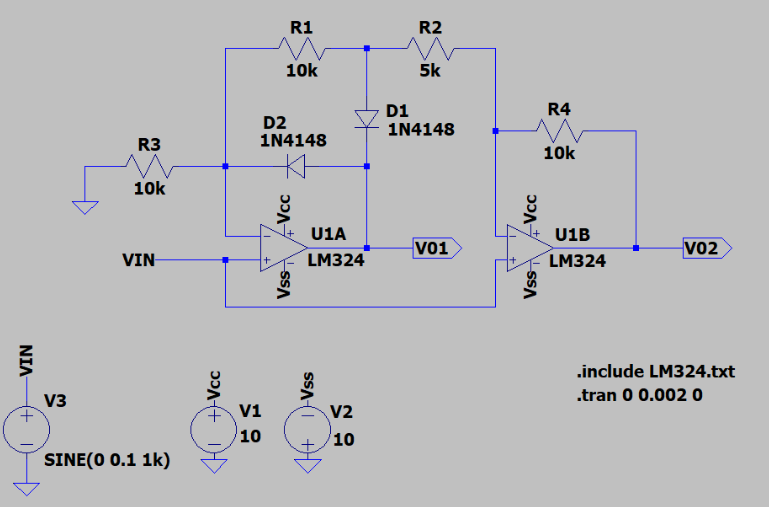
\includegraphics[width=0.5\linewidth]{c3simulacion.png}
     \caption{ Simulación del C3}
     \label{fig:enter-label}
 \end{figure}

\vspace{1em}

  \begin{figure}[h!]
     \centering
     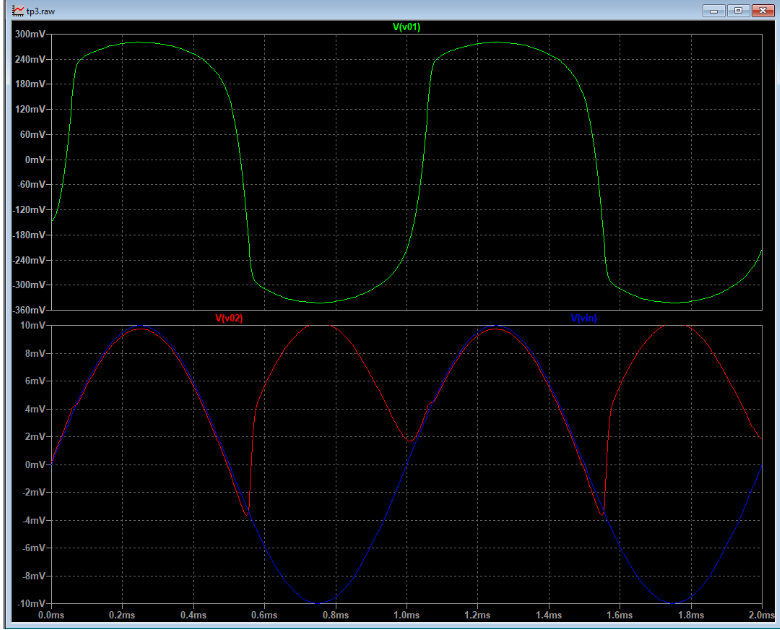
\includegraphics[width=0.5\linewidth]{c3vin001V.png}
     \caption{C3- señal de entrada $V_{in} = 0.1V$ con  $V_{o1}  y  V_{o2}$}
     \label{fig:enter-label}
 \end{figure}
 
  \begin{figure}[h!]
     \centering
     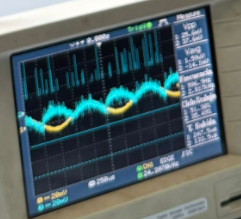
\includegraphics[width=0.4\linewidth]{c3vin10mVm.png}
     \caption{C3- señal de entrada $V_{in} = 0.01V  con V_{o2}$}
     \label{fig:enter-label}
 \end{figure}
 
 En esta figura (18), se puede notar que para señales muy pequeñas, menores al umbral del diodo, la señal
se rectifica de manera correcta.
 
 \vspace{1em}

  \begin{figure}[h!]
     \centering
     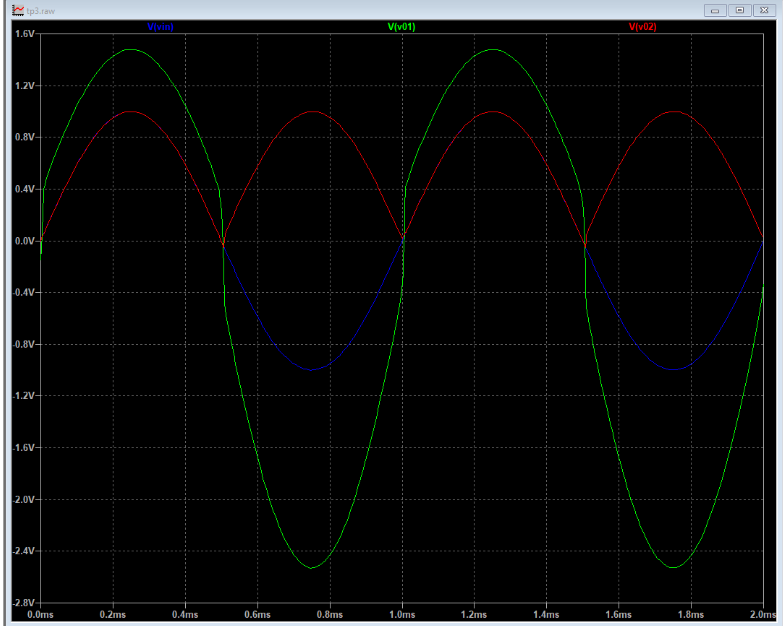
\includegraphics[width=0.5\linewidth]{c3vin1V.png}
     \caption{C3- señal de entrada $V_{in} = 1V$ con $V_{o1} y V_{o2}$}
     \label{fig:enter-label}
 \end{figure}
 
  \begin{figure}[h!]
     \centering
     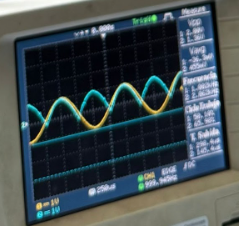
\includegraphics[width=0.4\linewidth]{c3vin1Vm.png}
     \caption{C3- señal de entrada $V_{in} = 1V  y V_{o2}$}
     \label{fig:enter-label}
 \end{figure}
 
 \vspace{1em}

  \begin{figure}[h!]
     \centering
     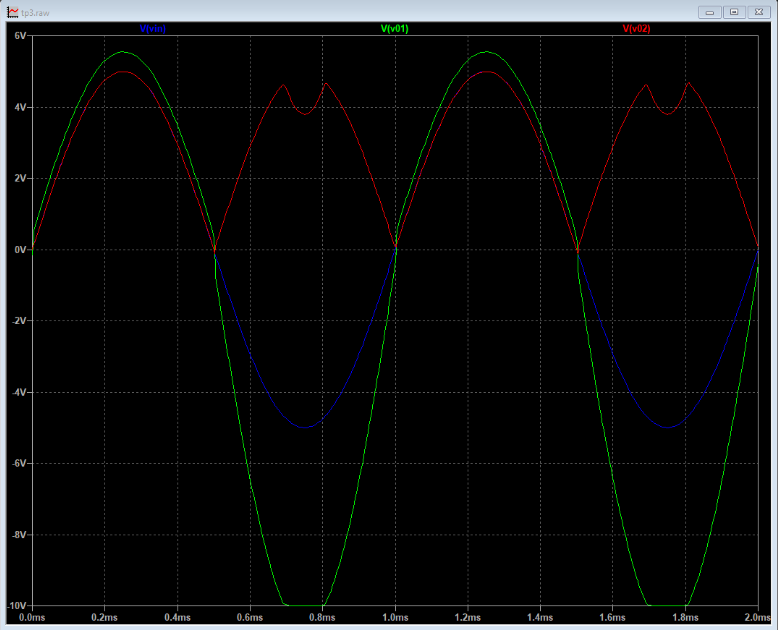
\includegraphics[width=0.5\linewidth]{c3vin5V.png}
     \caption{C3- señal de entrada $V_{in} = 5V$ con $V_{o1} y V_{o2}$}
     \label{fig:enter-label}
 \end{figure}
 
  \begin{figure}[h!]
     \centering
     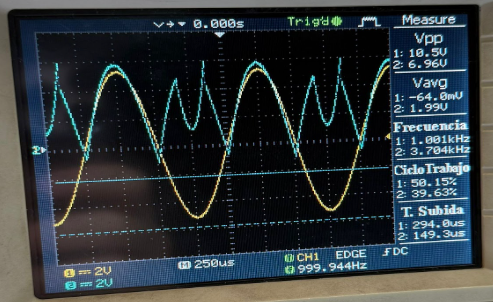
\includegraphics[width=0.4\linewidth]{c3vin5Vm.png}
     \caption{C3- señal de entrada $V_{in} = 5V  y V_{o2}$}
     \label{fig:enter-label}
 \end{figure}
 
 \vspace{1em}
 
 Se puede notar que hay un límite de tensión de $ V_{o1} $ para un correcto funcionamiento
del rectificador, cuando este se satura, la salida $V_{o2} $  se distorsiona. Como se tiene una
mayor ganancia en el semiciclo negativo de $V_{o1} $  es esperable que este sature primero y
distorsione la señal de salida. Por lo tanto, para tener un margen de seguridad razonable,
la tensión de entrada debe estar dentro del siguiente intervalo:  

\[ -3V < V_{in} < 3V \]
 
  \vspace{1em}

  \begin{figure}[h!]
     \centering
     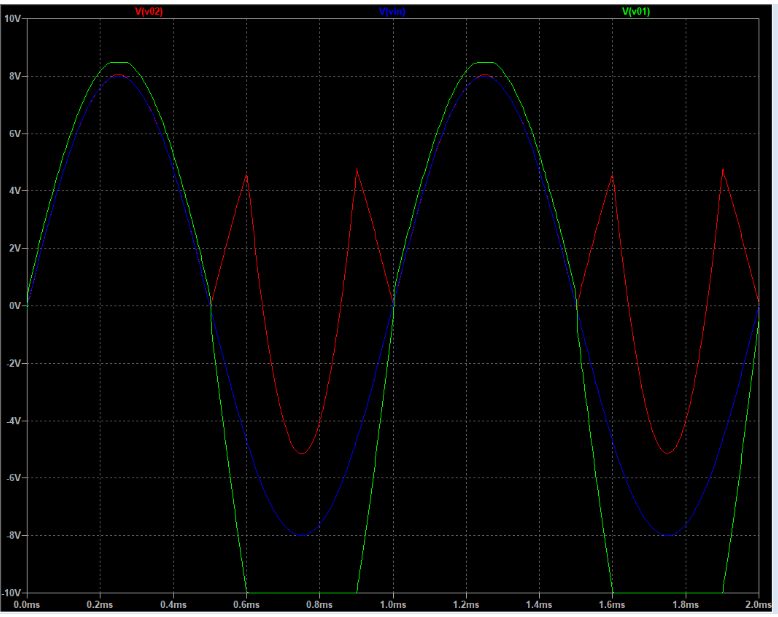
\includegraphics[width=0.5\linewidth]{c3vin8V.png}
     \caption{C3- señal de entrada $V_{in} = 8V$ y $V_{o1} y V_{o2}$}
     \label{fig:enter-label}
 \end{figure}

\vspace{1em}

Se puede apreciar en la figura 24 que para una tensión de entrada $V_{in} $ positiva, se tiene un
comportamiento lineal en el que la salida toma los mismos valores que la entrada,
es decir que el circuito tiene ganancia aproximadamente unitaria. 
Por otro lado, para una tensión $V_{in}$ negativa, se puede ver que el circuito se comporta como un
rectificador mientras esta se mantenga dentro de ciertos valores,  es necesario limitar el valor de la tensión de entrada teniendo en cuenta a qué
tensión se satura el AO, ya que cuando este se satura deja de rectificar correctamente


%\end{document}
